\documentclass{article}

\usepackage{geometry}
\usepackage{hyperref}

\usepackage{graphicx}
\graphicspath{ {./} }

\title {Khidmat: CS content development for TCF}

\author{
  Reeba Aslam\\ra02528 
}
\date{}  

\begin{document}
\maketitle

% Use first person plural (we, us) even if you did the Khidmat individually.

% An introduction of the project, no more than 2 sentences. Provide the highest level of detail only. Other details will come later.
% Typically, "This project is to <short description of porject> for/at <client>."
This project is to develop Computational Thinking related content in the CS curriculum being designed by FOCUS.\\

% About the client.
FOCUS is a non-profit organization with a goal to make Pakistan a leader in the technology field. We are philanthropists, tech specialists and academics passionate about developing a Computer Science curriculum and implementing it across schools and colleges in Pakistan.
The current project is focused on developing CS curriculum content for grades 6 to 8 for The Citizen's Foundation. \\

% About the project.
During the period of our work, we will be expected to develop content in form of chapters with associated exercises and learning outcomes, Teacher’s guide for each chapter with lesson plans and further suggestions for in-class activities that aid in delivering content and provide any additional material in the form of e.g., slides, programs, etc. that reinforces the learning outcomes if required.\\

% About the plan of work.
Apart from staff meetings in the first few weeks which were to ensure alignment of expected outcomes and deliverables, our physical presence is not required, however, in case of any issues or concerns, we will be engaging with the FOCUS staff. 
Moreover, we have been grouped with a FOCUS staff member with whom we can discuss content development regularly. Weekly updates will be shared via dropbox. The expected commitment is for approximately 160 hours – distributed into roughly 20 hours over 8 weeks. The final delivered content will be reviewed in the first week of August.

% Copy-paste this section with necessary modifcations for each week.
\newpage % Start the report for each week on a new page.
\section*{Week 1: 1--3 June, 2018}

% A summary, maximum 2 sentences, of this week's activities.
We had selected Hamiltonian Graphs as the first topic and spent time developing content for that.\\

\begin{tabular}{|l|l|l|l|}
    \hline
  Item 	& Activity & Time & ID \\\hline\hline
  1	& Searching for suitable Puzzles & 8 hrs & ra02528 \\\hline
  2	& Writing Content and Solution to Puzzles & 5 hrs & ra02528 \\\hline
  3	& Designing Class Activity & 2 hrs & ra02528 \\\hline
\end{tabular}\\


The total time spent on the Khidmat this week is as follows.

\begin{tabular}{|l|l|}
  \hline
  ID & Total Hours\\\hline\hline
  ra02528 & 10 hours\\\hline
\end{tabular}

\newpage % Start the report for each week on a new page.
\section*{Week 2: 4--10 June, 2018}
This week we started work on Exhaustive Search and Backtracking.\\

\begin{tabular}{|l|l|l|l|}
  \hline
  Item 	& Activity & Time & ID \\\hline\hline
  1	& Searching for suitable Puzzles(Exhaustive Search) & 6 hrs & ra02528 \\\hline
  2	& Searching for suitable Puzzles(Backtracking) & 2 hrs & ra02528 \\\hline
  3	& Writing Content and Solution to Puzzles (Exhaustive Search)& 8 hrs & ra02528 \\\hline
  4	& Writing Content and Solution to Puzzles (Backtracking)& 1 hrs & ra02528 \\\hline
  5	& Creating Illustrations & 3 hrs & ra02528 \\\hline
\end{tabular}\\

The total time spent on the Khidmat this week is as follows.

\begin{tabular}{|l|l|}
  \hline
  ID & Total Hours\\\hline\hline
  ra02528 & 20 hours\\\hline
\end{tabular}

\newpage % Start the report for each week on a new page.
\section*{Week 3: 11--17 June, 2018}
Last week's work needed quite many fixes which were pointed out in the weekly meeting. Our idea of a teacher's guide was not accurate and the chapters we designed needed to be more descriptive of the topic also having a few examples. Hence, this week we continued work on Exhaustive Search and added more content with extra puzzles.
\\

\begin{tabular}{|l|l|l|l|}
  \hline
  Item 	& Activity & Time & ID \\\hline\hline
  1	& Searching for suitable Puzzles /Examples & 4 hrs & ra02528 \\\hline
  2	& Adding additional content & 10 hrs & ra02528 \\\hline
  3	& Creating Illustrations & 6 hrs & ra02528 \\\hline
\end{tabular}\\

The total time spent on the Khidmat this week is as follows.

\begin{tabular}{|l|l|}
  \hline
  ID & Total Hours\\\hline\hline
  ra02528 & 20 hours\\\hline
\end{tabular}

\newpage % Start the report for each week on a new page.
\section*{Week 4: 18--24 June, 2018}
Resumed working on Backtracking and improved the chapter as done last week.\\


\begin{tabular}{|l|l|l|l|}
  \hline
  Item 	& Activity & Time & ID \\\hline\hline
  1	& Searching for suitable Puzzles/Examples & 2.5 hrs & ra02528 \\\hline
  2	& Writing content & 10.5 hrs & ra02528 \\\hline
  5	& Creating Illustrations & 7 hrs & ra02528 \\\hline
\end{tabular}\\

The total time spent on the Khidmat this week is as follows.

\begin{tabular}{|l|l|}
  \hline
  ID & Total Hours\\\hline\hline
  ra02528 & 20 hours\\\hline
\end{tabular}


\newpage % Start the report for each week on a new page.
\section*{Week 5: 25 June, 2018--1 July, 2018}
Updated Exhaustive Search and Backtracking on getting further feedback and developed Teacher's Guide for Exhaustive Search.\\


\begin{tabular}{|l|l|l|l|}
  \hline
  Item 	& Activity & Time & ID \\\hline\hline
  1	& Updating Exhaustive Search and Backtracking Chapters & 1 hrs & ra02528 \\\hline
  2	& Developing Teacher's Guide & 12 hrs & ra02528 \\\hline
  3	& Creating Illustrations for Teacher's Guide & 3 hrs & ra02528 \\\hline
\end{tabular}\\

The total time spent on the Khidmat this week is as follows.

\begin{tabular}{|l|l|}
  \hline
  ID & Total Hours\\\hline\hline
  ra02528 & 16 hours\\\hline
\end{tabular}

\newpage % Start the report for each week on a new page.
\section*{Week 6: 2 July, 2018--8 July, 2018}
Created Teacher's Guiude for backtracking.\\


\begin{tabular}{|l|l|l|l|}
  \hline
  Item 	& Activity & Time & ID \\\hline\hline
  1	& Developing Teacher's Guide & 11 hrs & ra02528 \\\hline
  2	& Creating Illustrations for Teacher's Guide & 5 hrs & ra02528 \\\hline
\end{tabular}\\

The total time spent on the Khidmat this week is as follows.

\begin{tabular}{|l|l|}
  \hline
  ID & Total Hours\\\hline\hline
  ra02528 & 16 hours\\\hline
\end{tabular}

\newpage % Start the report for each week on a new page.

\section*{Week 7: 9 July, 2018--15 July, 2018}
Worked on developing content for "Invariants" and created its teacher's guide.\\


\begin{tabular}{|l|l|l|l|}
  \hline
  Item 	& Activity & Time & ID \\\hline\hline
  1	& Searching for suitable Puzzles/Examples & 2 hrs & ra02528 \\\hline
  2	& Writing content & 13 hrs & ra02528 \\\hline
  3	& Developing Teacher's Guide & 12 hrs & ra02528 \\\hline
  4	& Creating Illustrations for Chapter &  2 hrs & ra02528 \\\hline
  5	& Creating Illustrations for Teacher's Guide & 1 hr & ra02528 \\\hline
\end{tabular}\\

The total time spent on the Khidmat this week is as follows.

\begin{tabular}{|l|l|}
  \hline
  ID & Total Hours\\\hline\hline
  ra02528 & 30 hours\\\hline
\end{tabular}


\newpage % Start the report for each week on a new page.

\section*{Week 8 and 9: 16 July, 2018-- 29 July, 2018}
A full chapter on Graph theory topics and its teacher's guide were developed these weeks.\\


\begin{tabular}{|l|l|l|l|}
  \hline
  Item 	& Activity & Time & ID \\\hline\hline
  1	& Writing content & 25 hrs & ra02528 \\\hline
  2	& Developing Teacher's Guide & 1 hr & ra02528 \\\hline
  3	& Creating Illustrations & 4 hr & ra02528 \\\hline
\end{tabular}\\

The total time spent on the Khidmat this week is as follows.

\begin{tabular}{|l|l|}
  \hline
  ID & Total Hours\\\hline\hline
  ra02528 & 30 hours\\\hline
\end{tabular}

\newpage
\section*{Conclusion}

% Remind the reader about the project. Summarise your activities over the course of the project.
%Our project was to build a new testing system for Habib University to replace ACCUPLACER for its entrance examination. We started by meeting all the stakeholders to understand their expectations from the new system. We then identified the necessary tools to build the required system and trained ourselves on them. Development and testing were carried out in collaboration with the IT team so that any shortcomings were identified and catered to as we went along. The system was then deployed and officers from the Admissions Team were trained to use it.

Our project was to develop content on Computational Thinking module of the CS curriculum being designed by Focus. We worked on specific topics every week. In the first few weeks, we met up with the staff to discuss the work we were doing so they could provide feedback. Their feedbacks were then incorporated into the work. All the chapters were designed along with the teacher's guide which were shared with our supervisor through a folder on Dropbox.

\newpage
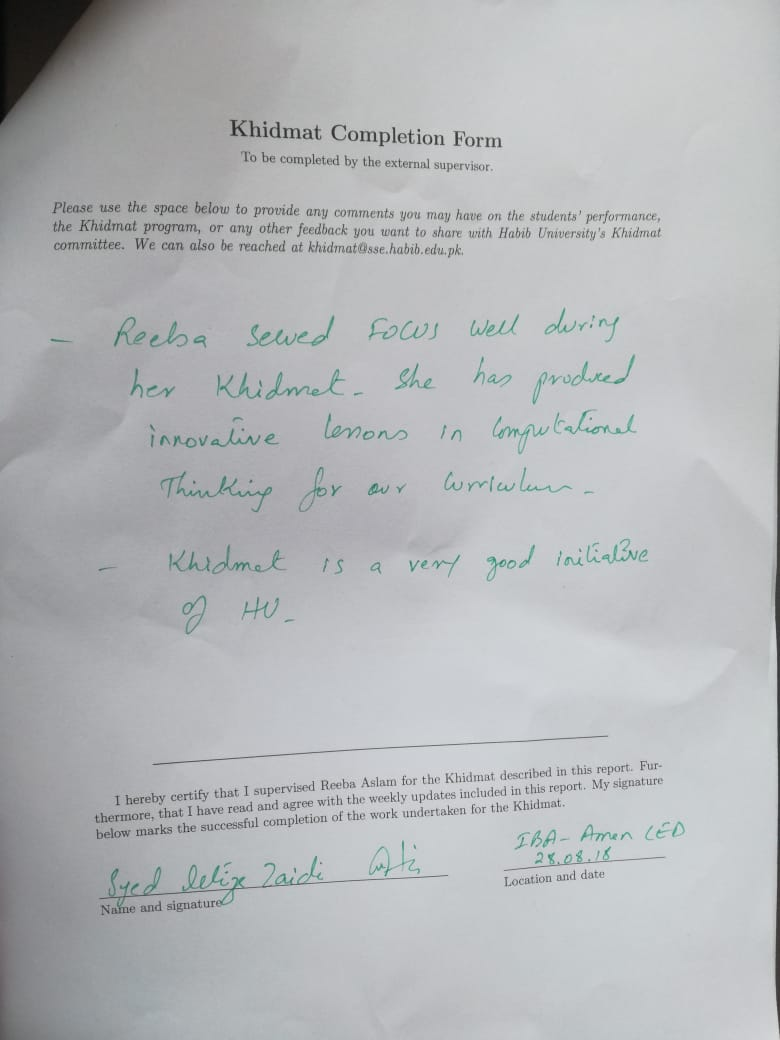
\includegraphics[width=\textwidth]{lastPage}

% Show your external supervisor your report, especially the weekly upates; have them sign a printed copy of this page; scan the signed page; and include the scanned page in this document as an image.


\end{document}
